\newsection
\section{Технический проект}
\subsection{Общие сведения о программной системе}

Необходимо спроектировать и разработать веб-платформу для анализа и визуализации статистических данных киберспортивной игры Counter-Strike 2.

Разрабатываемая программная система предназначена для предоставления комплексного инструмента анализа данных, который позволит игрокам, тренерам и аналитикам изучать подробную статистику матчей, улучшая таким образом свои стратегии и игровые навыки. Платформа предоставит интерактивный пользовательский интерфейс для визуализации данных, позволяя пользователям глубоко погружаться в аналитику матчей.

Основной принцип работы системы заключается в обработке .dem файлов матчей CS2 для извлечения детальных игровых метрик и последующем представлении их через графики, диаграммы и интерактивные отчеты. Пользователи смогут просматривать прогнозы на матч и статистику, такую как точность стрельбы, K/D Ratio, использование гранат и прочее, чтобы оценить силу команды и принять обоснованные решения.

Одним из ключевых компонентов программной системы является база данных для хранения извлеченной статистики матчей и команд. Кроме того, будет реализован функционал машинного обучения для предоставления прогнозов исходов матчей, основанных на исторических данных.

Целью разработки данной программной системы является создание эффективного инструмента анализа данных в киберспорте, который поможет повысить конкурентоспособность игроков и команд на международной арене, способствуя развитию киберспорта как спортивной дисциплины.


\subsection{Проектирование архитектуры программной системы}
\subsubsection{Выбор архитектурного стиля и паттернов проектирования}
Для разработки веб-платформы анализа и визуализации статистических данных CS2 был выбран микросервисный подход.[12] Такой стиль архитектуры подразумевает разбиение функционала системы на отдельные сервисы, каждый из которых отвечает за свою узкоспециализированную задачу.[13] Это обеспечивает гибкость в развертывании и масштабировании, упрощает поддержку и обновление компонентов системы без необходимости внесения изменений во все сервисы сразу, а только в конкретный.[14]

В качестве центрального входа в систему будет использоваться \textbf{API Gateway Pattern}, что позволит унифицировать обработку входящих запросов, распределение нагрузки, обеспечение безопасности и предоставление единой точки входа для клиентских приложений.[15]

Для взаимодействия с клиентами будет использоваться \textbf{REST API}, что гарантирует легкость интеграции и стандартизированное общение между сервисами.[16] REST API идеально подходит для микросервисной архитектуры за счет своей бесшовной и эффективной коммуникации.[17][18] А так же возможностью предоставления внешнего взаимодействия с сервером.

Все данные, передаваемые между клиентом и сервером, будут защищены с использованием \textbf{HTTPS}, обеспечивая конфиденциальность, целостность передачи данных и защиту от муждуузловых атак.[19]

Для повышения производительности и снижения нагрузки на базу данных будет использоваться подход \textbf{Cache-Aside} в сочетании с \textbf{Redis}.[20] Это позволит хранить часто запрашиваемые данные в быстром кеше, что существенно ускорит время их доставки конечному пользователю.[21]

Для асинхронного обмена сообщениями между различными микросервисами в системе будет применяться \textbf{RabbitMQ}. Этот брокер сообщений позволит надежно обрабатывать задачи в фоновом режиме, улучшая производительность и масштабируемость системы, обеспечивая отказоустойчивость и балансировку нагрузки при высоких объемах обмена данными.[22]

Данная архитектура обеспечивает всей системе необходимую гибкость для развития и масштабирования, а также повышает надежность и отказоустойчивость приложения при больших нагрузках.

Архитектура всей системы представлена на рисунке \ref{fig:-architecture}.
\begin{figure}
	\centering
	\includegraphics[width=0.9\linewidth]{"images/Архитектура"}
	\caption{Архитектура программной системы}
	\label{fig:-architecture}
\end{figure}

\subsubsection{Обоснование выбора средств для работы с базой данных}

Основной  системой управления базой данных для хранения данных в системе будет выступать \textbf{PostgreSQL}. Эта СУБД была выбрана за её надежность, масштабируемость и поддержку сложных запросов, что является критически важным для аналитических запросов, связанных с большими объемами данных.[23] PostgreSQL будет использоваться для хранения всех основных данных системы в SQL формате.[24]

На рисунке \ref{fig:-bd} представлена схема базы данных.
\begin{figure}
	\centering
	\includegraphics[width=1\linewidth]{"images/База данных"}
	\caption{Схема базы данных}
	\label{fig:-bd}
\end{figure}

Redis будет использоваться как вспомогательная система для кеширования часто запрашиваемых данных. Это позволит значительно ускорить время отклика системы, уменьшить нагрузку на основную базу данных и предоставить пользователям актуальную информацию с минимальной задержкой. Redis должна использоваться для кеширования данных в формате ключ-значение, где ключом будет выступать хеш объекта, а значением сам данный объект.

\subsubsection{Описание микросервисов}

Веб-платформа будет включать в себя следующие микросервисы:

\begin{itemize}
	\item \textbf{API Gateway:} Является точкой входа в систему, маршрутизирует запросы к соответствующим сервисам. Связан со всеми сервисами.
	\item \textbf{Сервис поиска информации о турнирах:} Отвечает за предоставление актуальных данных о киберспортивных турнирах. Сервис взаимодействует с базой данных и API сторонних платформ для обновления и поддержания в актуальном состоянии информации о предстоящих и прошедших турнирах.
	\item \textbf{Сервис анализа .dem файла:} Загружает и анализирует загруженные .dem файлы, извлекает из матча основные статистические данные для добавления их в базу данных и обработки другими сервисами.
	\item \textbf{Сервис предоставления данных:} Управляет предоставлением данных для разных разделов. Сервис взаимодействует с базой данных для получения, обработки и отправки информационных и статистических данных в нужном формате.
	\item \textbf{Сервис поиска:} Реализует функциональность поиска по всем сегментам данных платформы. Интегрирован с другими сервисами и предоставляет пользователю удобный поиск по игрокам, командам и турнирам.
	\item \textbf{Сервис прогнозирования:} Использует машинное обучение и алгоритмы прогнозирования для предсказания исходов матчей. Анализирует исторические данные и текущие тенденции для генерации прогнозов.
	\item \textbf{Брокер сообщений (RabbitMQ):} Обеспечивает надежную передачу сообщений между сервисами, поддерживает распределенные транзакции и асинхронное взаимодействие в микросервисной архитектуре.
	\item \textbf{Prometheus:} Используется для мониторинга работы сервисов, сбора метрик и уведомления о проблемах, позволяя оперативно реагировать на сбои и изменения в работе системы.[25]
\end{itemize}

На рисунке \ref{fig:-conceptual_classes} представлены концептуальные классы backend части веб-платформы.
\begin{figure}
	\centering
	\includegraphics[width=0.9\linewidth]{"images/Концептуальные классы"}
	\caption[Концептуальные классы backend части веб-платформы]{Концептуальные классы backend части веб-платформы}
	\label{fig:-conceptual_classes}
\end{figure}

\subsubsection{Планирование докеризации и оркестрации сервисов}

Для достижения высокой отказоустойчивости, удобства в развертывании и эффективного масштабирования, развертывание каждого микросервиса веб-платформы будет выполнено в контейнере Docker. Каждый контейнер в себе будет включать требуемое ядро системы, используемые библиотеки и настройки окружения для запуска данного микросервиса.[26] Это позволит обеспечить изоляцию зависимостей между частями платформы и согласованность окружений независимо от инфраструктуры развертывания.

Оркестрация контейнеров будет производиться с помощью Kubernetes, что гарантирует автоматизацию развертывания, масштабирования и управления приложениями контейнеров. Kubernetes обеспечивает балансировку нагрузки, самовосстановление сервисов при их ошибках, автоматическое распределение ресурсов и управление конфигурацией.[27]

Вся инфраструктура веб-платформы будет развернута в облаке Yandex Cloud, что обеспечит высокую доступность сервисов и возможности простой интеграции с другими облачными сервисами.

\subsubsection{Описание REST API микросервисов}

\begin{xltabular}{\textwidth}{|X|X|X|X|}
	\caption{Сервис API Gateway}\label{apigateway:table}\\ \hline
	\thead{HTTP-\\метод} & \thead{Описание} & \thead{Входные\\параметры} & \thead{Пример\\JSON ответа} \\ \hline
	\thead{1} & \thead{2} & \thead{3} & \thead{4} \\ \hline
	\endfirsthead
	\continuecaption{Продолжение таблицы \ref{apigateway:table}} \hline
	\thead{1} & \thead{2} & \thead{3} & \thead{4} \\ \hline
	\endhead
	POST /api/ & Маршрутизация запросов & \{"service": "string", "endpoint": "string", "data": "object"\} & \{"status": "success", "data": "object"\} \\ \hline
	GET /api/ & Получение данных от сервисов & \{"service": "string", "endpoint": "string", "params": "object"\} & \{"status": "success", "data": "object"\} \\ \hline
\end{xltabular}

\begin{xltabular}{\textwidth}{|X|X|X|X|}
	\caption{Сервис поиска информации о турнирах}\label{tournamentsearch:table}\\ \hline
	\thead{HTTP-\\метод} & \thead{Описание} & \thead{Входные\\параметры} & \thead{Пример\\JSON ответа} \\ \hline
	\thead{1} & \thead{2} & \thead{3} & \thead{4} \\ \hline
	\endfirsthead
	\continuecaption{Продолжение таблицы \ref{tournamentsearch:table}} \hline
	\thead{1} & \thead{2} & \thead{3} & \thead{4} \\ \hline
	\endhead
	POST api/Background
	ServiceController
	/start-team-update & Запуск фонового получения данных команд & Нет  & \{"result": "string"\} \\ \hline
	POST api/Background
	ServiceController
	/start-tournament-update & Запуск фонового получения данных турниров и стадий & Нет  & \{"result": "string"\} \\ \hline
	POST api/Background
	ServiceController
	/start-match-update & Запуск фонового получения данных матчей & Нет  & \{"result": "string"\} \\ \hline
	POST api/Background
	ServiceController
	/start-stats-update & Запуск фонового получения данных статистики & Нет  & \{"result": "string"\} \\ \hline
	POST api/Background
	ServiceControlle
	/stop/:serviceName & Запуск фонового получения данных команд & \{"serviceName": "string"\}  & \{"result": "string"\} \\ \hline
\end{xltabular}

\begin{xltabular}{\textwidth}{|X|X|X|X|}
	\caption{Сервис анализа .dem файла}\label{demfileanalysis:table}\\ \hline
	\thead{HTTP-\\метод} & \thead{Описание} & \thead{Входные\\параметры} & \thead{Пример\\JSON ответа} \\ \hline
	\thead{1} & \thead{2} & \thead{3} & \thead{4} \\ \hline
	\endfirsthead
	\continuecaption{Продолжение таблицы \ref{demfileanalysis:table}} \hline
	\thead{1} & \thead{2} & \thead{3} & \thead{4} \\ \hline
	\endhead
	POST api/analyze/upload & Загрузка .dem файла & \{"file": "binary"\} & \{"status": "string"\} \\ \hline
	POST api/analyze/
	analyze & Анализ загруженного файла & \{"tournament\_id": "int", "stage\_id": "int", "team1\_id": "int", "team2\_id": "int", "map\_id": "int", "file\_name": "string"\} & \{"status": "string"\} \\ \hline
\end{xltabular}

\begin{xltabular}{\textwidth}{|X|X|X|X|}
	\caption{Сервис поиска}\label{searchservice:table}\\ \hline
	\thead{HTTP-\\метод} & \thead{Описание} & \thead{Входные\\параметры} & \thead{Пример\\JSON ответа} \\ \hline
	\thead{1} & \thead{2} & \thead{3} & \thead{4} \\ \hline
	\endfirsthead
	\continuecaption{Продолжение таблицы \ref{searchservice:table}} \hline
	\thead{1} & \thead{2} & \thead{3} & \thead{4} \\ \hline
	\endhead
	GET api/search/ & Поиск по запросу & \{"query": "string"\} & \{"results": [\{"Players": [object]\}, \{"Teams": [object]\}, \{"Tournaments": [object]\}] \} \\ \hline
\end{xltabular}

\begin{xltabular}{\textwidth}{|X|X|X|X|}
	\caption{Сервис прогнозирования}\label{predictionservice:table}\\ \hline
	\thead{HTTP-\\метод} & \thead{Описание} & \thead{Входные\\параметры} & \thead{Пример\\JSON ответа} \\ \hline
	\thead{1} & \thead{2} & \thead{3} & \thead{4} \\ \hline
	\endfirsthead
	\continuecaption{Продолжение таблицы \ref{predictionservice:table}} \hline
	\thead{1} & \thead{2} & \thead{3} & \thead{4} \\ \hline
	\endhead
	POST api/prediction
	/predict & Генерация прогноза на матч & \{"matchId": "int"\} & \{"prediction": \{"winProbability": "float"\} \} \\ \hline
\end{xltabular}

\begin{xltabular}{\textwidth}{|X|X|X|X|}
	\caption{Сервис предоставления данных}\label{dataservice:table}\\ \hline
	\thead{HTTP-\\метод} & \thead{Описание} & \thead{Входные\\параметры} & \thead{Пример\\JSON ответа}\\ \hline
	\thead{1} & \thead{2} & \thead{3} & \thead{4}\\ \hline
	\endfirsthead
	\continuecaption{Продолжение таблицы \ref{dataservice:table}} \hline
	\thead{1} & \thead{2} & \thead{3} & \thead{4}\\ \hline
	\endhead
	GET api/data
	/tournament
	/current & Получение будущих турниров & \{\} & \{"tournaments": ["object"]\}\\ \hline
	GET api/data
	/tournament
	/finished & Получение предыдущих турниров & \{\} & \{"tournaments": ["object"]\}\\ \hline
	GET api/data
	/tournamen
	t/:slug & Получение определенного турнира & \{"slug": "string"\} & \{"tournament": "object"\}\\ \hline
	GET api/data
	/match/finished & Получение предыдущих матчей & \{\} & \{"matches": ["object"]\}\\ \hline
	GET api/data
	/match/current & Получение будущих матчей & \{\} & \{"matches": ["object"]\}\\ \hline
	GET api/data
	/match/:slug & Получение конкретного матча & \{"slug": "string"\} & \{"match": "object"\}\\ \hline
	GET api/data
	/match
	/:slug/stats & Получение статистики конкретного матча & \{"slug": "string"\} & \{"statistics": "object"\}\\ \hline
	GET api/data
	/match/:slug
	/stats/:mapName & Получение статистики конкретной карты & \{"slug":"string"\, "mapName": "string"\} & \{"statistics": "object"\}\\ \hline
	GET api/data
	/player/ & Получение игроков & \{\} & \{"players": ["object"]\}\\ \hline
	GET api/data
	/team/ & Получение команд & \{\} & \{"teams": ["object"]\}\\ \hline
	GET api/data
	/player/:slug & Получение отдельной команды & \{"slug": "string"\} & \{"team": "object"\}\\ \hline
	GET api/data
	/team/:slug & Получение отдельного игрока & \{"slug": "string"\} & \{"player": "object"\}\\ \hline
	GET api/data
	/compare
	/players & Сравнение двух игроков & \{"player1Slug": "string"\,  "player2Slug": "string"\} & \{"comparison": \{"player1": "object", "player2": "object" \}\}\\ \hline
	GET api/data
	/compare
	/teams & Сравнение двух команд & \{"team1Slug": "string"\, "team2Slug": "string"\} & \{"comparison": \{"team1": "object", "team2": "object"\}\}\\ \hline
\end{xltabular}

\subsection{Обоснование выбора технологий проектирования и программных средств}
\subsubsection{Выбор используемых технологий и языков программирования}

\paragraph{API Gateway}

Для реализации данного микросервиса должен быть выбран язык C\# с библиотекой Ocelot для реализации шлюзов и перенаправлений запросов API.[28]

\paragraph{Сервис поиска информации о турнирах}

Для реализации данного микросервиса должен быть выбран язык C\# с использованием библиотек AutoMapper - для реализации мапинга считываемых сущностей из открытых источников и преобразования их в сущности используемые внутри системы, Entity Framework Core - для реализации работы с базами данных, используя объектноориентированный подход, Newtonsoft.Json - для преобразования получаемых JSON файлов в сущности DTO.[29][30][31]

\paragraph{Сервис поиска информации о турнирах}

Для реализации данного микросервиса должен быть выбран язык Go, так как он предлагает высокую производительность и эффективность в обработке и анализе низкоуровневых данных, таких как  бинарные файлы .dem записей матчей, благодаря своим встроенным средствам для параллельной обработки.[32][33][34] Так же должна использоваться библиотека demoinfocs-golang - библиотека для разбора и анализа .dem файлов игры Counter-Strike 2.[35]

\paragraph{Сервис предоставления данных}

Для реализации данного микросервиса должен быть выбран язык C\# с использованием библиотек Entity Framework Core - для реализации работы с базами данных, AutoMapper - для реализации мапинга сущностей из базы данных в сущности DTO (Data Transfer Object) отправляемые на frontend часть веб-платформы.

\paragraph{Сервис поиска}

Для реализации данного микросервиса должен быть выбран язык C\# с использованием библиотек Entity Framework Core - для реализации работы с базами данных и библиотеки AutoMapper - для реализации мапинга сущностей из базы данных в сущности DTO (Data Transfer Object) отправляемые на frontend часть веб-платформы.

\paragraph{Сервис прогнозирования}

Для реализации данного микросервиса должен быть выбран язык Python из-за его превосходной поддержки библиотек машинного обучения и аналитики данных.[36] Для данного модуля должны использоваться библиотека sklearn - для подготовки датасета для обучения нейронной сети, tensorflow - для непосредственно создания нейронной сети и ее обучения.[37]

\paragraph{Брокер сообщений (RabbitMQ)}

Для реализации взаимодействия между микросервисами через брокер сообщений будет использоваться RabbitMQ. Для работы с RabbitMQ должен быть выбран язык C\# с библиотекой RabbitMQ.Client, предоставляющей удобный API для взаимодействия с RabbitMQ.

\paragraph{Prometheus}

Для мониторинга и алертинга инфраструктуры будет использоваться Prometheus. Он позволит собирать метрики с различных сервисов и узлов, а также устанавливать алерты на основе собранных данных.[38] В микросервисах на C\# для экспорта метрик в Prometheus должна использоваться библиотека prometheus-net.

\paragraph{React}

React - это JavaScript библиотека, разработанная компанией Facebook, предназначенная для создания пользовательских интерфейсов веб-приложений.[39] Она позволяет разрабатывать динамические и интерактивные веб-страницы, обладающие высокой производительностью и масштабируемостью.[40]

Одной из ключевых особенностей React является использование компонентного подхода к созданию интерфейса. Приложение строится из небольших и независимых компонентов, каждый из которых отвечает за определенную часть пользовательского интерфейса. Это позволяет создавать чистый и упорядоченный код, легко поддерживаемый и расширяемый.

Ещё одним важным преимуществом React является использование виртуального DOM (Document Object Model). React создает виртуальное представление DOM в памяти, которое затем сравнивается с реальным DOM и обновляется только та часть, которая изменилась. Это позволяет увеличить производительность приложения и улучшить пользовательский опыт.
React также предоставляет множество инструментов и библиотек для управления состоянием приложения, маршрутизации, тестирования и других задач. Экосистема React очень развита, что делает его популярным выбором для разработки веб-приложений.

Во время разработки веб-платформы должны быть реализованы следующие компоненты для создания полноценной структуры и выполнения поставленных требований в пункте 2.3 технического задания:
\begin{itemize}
	\item \textbf{Компонент отображения статистики по всем картам отдельного игрока:} этот компонент предназначен для отображения статистики игры отдельного игрока по различным картам. Он должен включать среднюю оценку игрока на карте, количество сыгранных карт,  и средние данные, такие как среднее число убийств и урона за раунд.
	\item \textbf{Таблица игроков команды в матче:} таблица, представляющая собой список всех игроков участвующих в матче с их ключевыми статистическими данными для данного матча. Это может включать K/D/A (убийства/смерти/ассисты), разницу между убийствами и смертями, рейтинг и форму игрока в данном матче, и другие данные.
	\item \textbf{Компонент вывода статистики команд за последние 6 месяцев на всех картах:} компонент, который показывает собранные данные о производительности команды на различных картах за последние полгода. Информация представлена в виде процента побед на отдельных картах, среднее число убийств и урона за раунд и отображение статуса победы в последних 5 играх на каждой карте.
	\item \textbf{Компонент сравнения статистики команд и игроков по основным метрикам:} данный компонент предоставляет сравнительный анализ между командами или игроками, позволяя пользователям видеть различия в ключевых статистических показателях. Может быть полезен для анализа формы команд перед матчами. В нем выбранные для сравнения команды или игроки представлены в виде таблицы со всеми метриками, которые попарно сравниваются и выделяются больший из них.
	\item \textbf{Блок формирования одинаковой структуры для всех используемых блоков в системе:} данный компонент является основой для стандартизации внешнего вида и структуры различных компонентов на сайте. Это помогает в обеспечении консистентности пользовательского интерфейса и улучшает общий пользовательский опыт.
	\item \textbf{Компонент отображения команды со списком игроков:} компонент для отображения команды и списка игроков в команде, включая их аватары, название команды и прочее. Данный компонент используется для предоставления обзора состава команды в матчах или турнирах.
\end{itemize}

\subsubsection{Выбор программного обеспечения}

Разработка веб-платформы для анализа и визуализации статистических данных игры Counter-Strike 2 требует продуманного подхода к выбору аппаратного обеспечения. Основные критерии выбора – масштабируемость, надежность, и производительность системы. В качестве основы для реализации инфраструктуры выбраны современные технологии контейнеризации, оркестрации, управления очередями сообщений и мониторинга: Docker, Kubernetes, RabbitMQ, и Prometheus.

Важным аспектом является решение о запуске всей инфраструктуры в облачной среде, что обеспечивает высокую гибкость, масштабируемость и доступность ресурсов. Облачные сервера Yandex Cloud, на которых будет развернута система, будут работать под управлением операционной системы Linux, что гарантирует стабильность работы и широкие возможности для настройки системы.[41]

\subsubsection{Docker}

Docker предоставляет легковесную и удобную платформу для создания, развертывания и управления контейнерами. Контейнеризация упрощает процесс разработки, тестирования и развертывания приложений, позволяя запускать приложения и их зависимости в изолированных средах. В контексте выбора аппаратного обеспечения это означает возможность оптимизации использования ресурсов и увеличение эффективности за счет развертывания на облачных серверах с поддержкой Docker.

На рисунке \ref{fig:-Docker} представлена архитектура платформы Docker.
\begin{figure}
	\centering
	\includegraphics[width=0.9\linewidth]{"images/Docker"}
	\caption{Архитектура платформы Docker}
	\label{fig:-Docker}
\end{figure}

Данная архитектура состоит из следующих элементов:
\begin{enumerate}
	\item Infrastructure (Инфраструктура): Это физические серверы или виртуальные машины, на которых развёрнуты контейнеризированные приложения. Инфраструктура предоставляет вычислительные ресурсы, такие как процессор, память, дисковое пространство и сеть.
	\item Host Operating System (Хостовая операционная система): Это операционная система, установленная на инфраструктуре. Она управляет аппаратными ресурсами и предоставляет базовые функции для работы контейнеров.
	\item Docker: Docker — это платформа для контейнеризации, которая позволяет разрабатывать, отправлять и запускать приложения в изолированных контейнерах. Docker использует технологии виртуализации на уровне операционной системы, такие как cgroups и namespaces, для изоляции контейнеров.
	\item Containerized Applications (Контейнеризированные приложения): Это приложения, упакованные в контейнеры Docker. Контейнеры включают все необходимые зависимости, библиотеки и конфигурации для работы приложения, что обеспечивает их портативность и изолированность.
\end{enumerate}

\subsubsection{Redis}

Redis — это база данных, размещаемая в памяти, которая используется, в основном, в роли кеша, находящегося перед другой, «настоящей» базой данных, вроде MySQL или PostgreSQL. Кеш, основанный на Redis, помогает улучшить производительность приложений. Он эффективно использует скорость работы с данными, характерную для памяти, и смягчает нагрузку центральной базы данных приложения, связанную с обработкой следующих данных:
\begin{itemize}
	\item Данные, которые редко меняются, к которым часто обращается приложение.
	\item Данные, не относящиеся к критически важным, которые часто меняются.
\end{itemize}

Примеры таких данных могут включать в себя сессионные кеши или кеши данных, а так же содержимое панелей управления — вроде списков лидеров и отчётов, включающих в себя данные, агрегированные из разных источников.

Рассмотрим, как работает Redis в качестве кеша на основе архитектуры представленной на рисунке \ref{fig:-Redis}.
\begin{figure}
	\centering
	\includegraphics[width=0.9\linewidth]{"images/Redis"}
	\caption{Пример работы Redis}
	\label{fig:-Redis}
\end{figure}

Пример работы при первом обращении к данным:
\begin{enumerate}
	\item Пользователь делает запрос к серверу (Шаг 1).
	\item Сервер проверяет наличие необходимых данных в Redis (Шаг 2).
	\item Если данных в кэше нет, сервер отправляет запрос к основной базе данных (Шаг 3).
	\item Основная база данных обрабатывает запрос и возвращает данные серверу (Шаг 4).
	\item Получив данные от основной базы данных, сервер сохраняет их в Redis для последующих запросов (Шаги 5-6).
	\item После сохранения данных в кеше они отправляются пользователю (Шаг 7).
\end{enumerate}

Пример работы при обращении к уже сохраненным данным в Redis:
\begin{enumerate}
	\item Пользователь делает запрос к серверу (Шаг 1).
	\item Данные находятся в кеше и возвращаются серверу (Шаг 5).
	\item Сервер отправляет данные пользователю (Шаг 7).
\end{enumerate}

Благодаря использованию кеширования удается уменьшить скорость получения данных при их повторном вызове до x10 раз.

\subsubsection{Kubernetes}

Kubernetes является мощной системой для автоматизации развертывания, масштабирования и управления контейнеризированными приложениями. В архитектуре веб-платформы Kubernetes обеспечивает высокую доступность, автоматическое масштабирование и балансировку нагрузки между контейнерами.[42] Для аппаратного обеспечения это подразумевает необходимость в выделенном или облачном сервере с достаточным количеством процессорного времени и оперативной памяти для поддержания кластера Kubernetes.

\subsubsection{RabbitMQ}

RabbitMQ, система управления очередями сообщений, играет ключевую роль в обеспечении асинхронной обработки данных и интеграции различных частей системы. Эффективное использование RabbitMQ позволяет распределить нагрузку, улучшить производительность приложения и обеспечить надежную обработку сообщений.[43] Аппаратное обеспечение должно соответствовать требованиям по пропускной способности и скорости обработки сообщений, что особенно важно при больших объемах данных. Сервер на котором будет находится данный сервис должен быть максимально отказоустойчивым, для исключения лавинного выхода из строя микросервисов.

На рисунке \ref{fig:-RabbitMQ} представлена работа RabbitMQ и системы управления очередями сообщений (message broker) в процессе передачи сообщений от производителя (publisher) к потребителю (consumer). \ref{fig:-RabbitMQ}.
\begin{figure}
	\centering
	\includegraphics[width=0.9\linewidth]{"images/RabbitMQ"}
	\caption{Пример работы RabbitMQ}
	\label{fig:-RabbitMQ}
\end{figure}

Схема состоит из следующих элементов:
\begin{enumerate}
	\item Publisher (Производитель): это модуль, который отправляет сообщения. В данном примере производитель публикует сообщение с ключом маршрутизации (routing key), равным "somekey".	
	\item Exchange (Обменник): обменник принимает сообщения от производителей и маршрутизирует их в очереди на основе ключа маршрутизации. Обменники могут быть разных типов (direct, fanout, topic, headers), что определяет правила маршрутизации сообщений. В данном примере обменник получает сообщение с ключом маршрутизации "somekey" и определяет, в какую очередь его направить.
	\item Queue (Очередь): очередь — это место, где сообщения хранятся до тех пор, пока они не будут получены потребителем. Очереди могут быть долговременными (persistent), чтобы сохраняться при перезапуске сервера RabbitMQ, или временными (transient), которые удаляются при перезапуске. В данном примере сообщение с ключом маршрутизации "somekey" попадает в определенную очередь.
	\item Consumer (Потребитель): потребитель получает сообщения из очереди и обрабатывает их. Потребители могут подтверждать получение сообщений (acknowledgements), чтобы уведомить RabbitMQ, что сообщение было успешно обработано. В данном примере потребитель извлекает сообщение из очереди и выполняет необходимые действия.
\end{enumerate}

\subsubsection{Prometheus}

Prometheus — система мониторинга и оповещения, которая позволяет собирать и анализировать метрики в реальном времени. Использование Prometheus обеспечивает возможность наблюдения за производительностью системы, оптимизации ресурсов и быстрого реагирования на возникающие проблемы. Аппаратное обеспечение должно обладать достаточным объемом хранилища для сбора и хранения данных метрик, а также процессорной мощностью для их обработки.

\subsection{Проектирование пользовательского интерфейса программной системы}
\subsubsection{Макеты пользовательского интерфейса}

На основании требований к пользовательскому интерфейсу, представленных в пункте 2.3 технического задания, был разработан графический интерфейс мобильного приложения, используя React с использованием библиотеки Material UI.[44] Разработанный интерфейс ориентирован на обеспечение легкости в использовании и удобного визуального представления статистических данных.

На рисунке \ref{fig:-teamPage} представлен макет страницы команды.
\begin{figure}
	\centering
	\includegraphics[width=0.95\linewidth]{"images/Страница команды"}
	\caption{Макет страницы команды}
	\label{fig:-teamPage}
\end{figure}

Макет содержит следующие элементы:
\begin{itemize}
	\item Название команды.
	\item Логотип команды.
	\item Статистика команды по картам.
	\item Список матчей команды.
	\item Состав команды.
\end{itemize}

На рисунке \ref{fig:-playerPage} представлен макет страницы игрока.
\begin{figure}
	\centering
	\includegraphics[width=0.95\linewidth]{"images/Страница игрока"}
	\caption{Макет страницы игрока}
	\label{fig:-playerPage}
\end{figure}

Макет содержит следующие элементы:
\begin{itemize}
	\item Никнейм игрока.
	\item Фото игрока.
	\item Статистика игрока по картам.
	\item Список матчей данного игрока.
	\item Основную информацию о игроке.
	\item Прочую статистику игрока.
\end{itemize}

На рисунке \ref{fig:-matchPage} представлен макет страницы матча.
\begin{figure}
	\centering
	\includegraphics[width=0.95\linewidth]{"images/Страница матча"}
	\caption{Макет страницы матча}
	\label{fig:-matchPage}
\end{figure}

Макет содержит следующие элементы:
\begin{itemize}
	\item Турнир и стадию для данного матча.
	\item Счет и названия команд матча.
	\item Основную информацию матча.
	\item Статистику игроков в данном матче по командам.
\end{itemize}

На рисунке \ref{fig:-tournamentPage} представлен макет страницы турнира.
\begin{figure}
	\centering
	\includegraphics[width=0.95\linewidth]{"images/Страница турнира"}
	\caption{Макет страницы турнира}
	\label{fig:-tournamentPage}
\end{figure}

Макет содержит следующие элементы:
\begin{itemize}
	\item Название турнира, логотип его дата.
	\item Список участвующих команд.
	\item Основную информацию турнира.
	\item Список матчей данного турнира.
\end{itemize}

\subsubsection{Компоненты пользовательского интерфейса}

Для создания фронтенд части веб-платформы полноценной структуры созданы следующие компоненты:

\paragraph{MiddleContent}

Компонент MiddleContent используется для отображения основной информации и содержимого страницы. Он включает в себя изменяемые заголовок, подзаголовок, аватар и дополнительное содержимое с возможностью указания ширины конечного блока. 

На рисунке \ref{fig:MiddleContent} представлен пример отображения компонента MiddleContent:
\begin{figure}
	\centering
	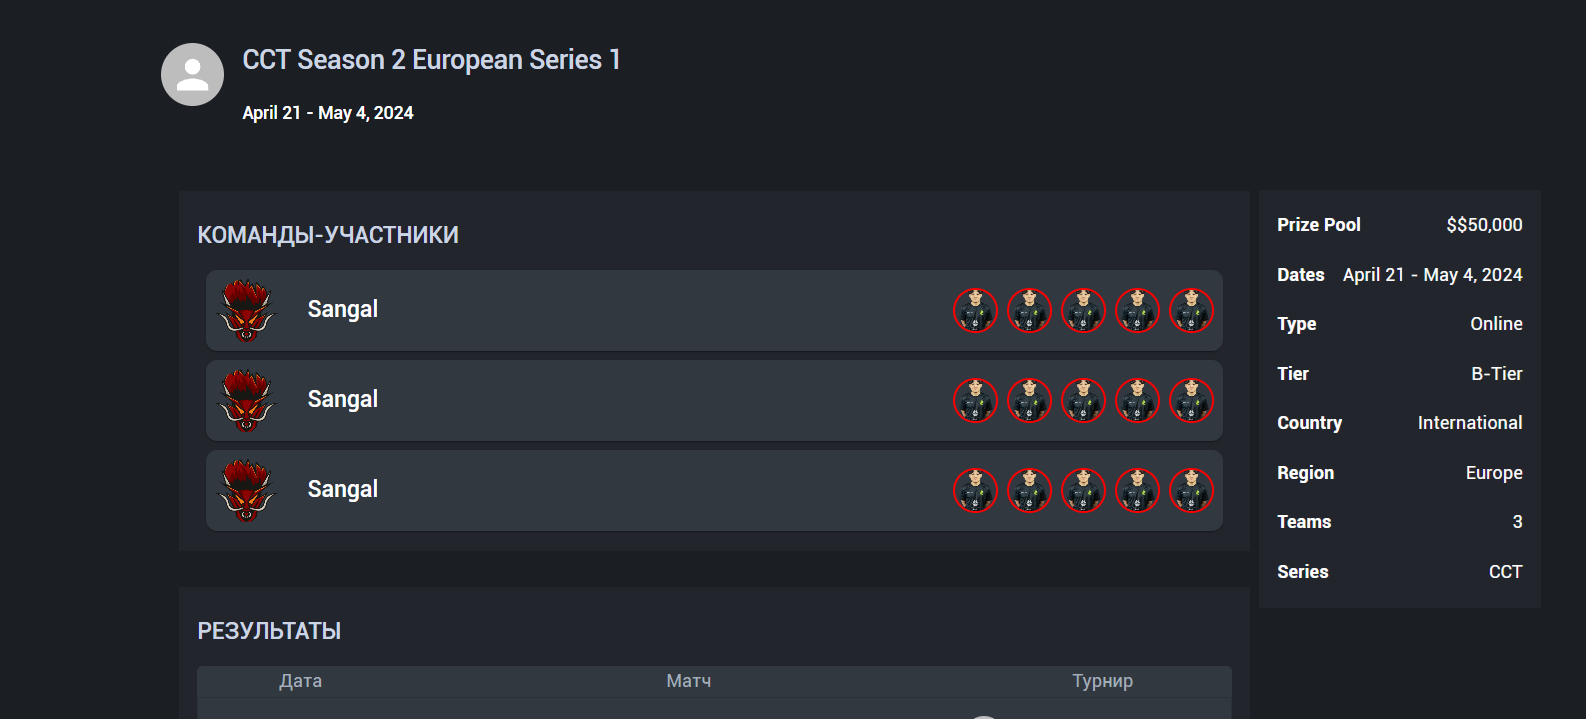
\includegraphics[width=0.95\linewidth]{images/MiddleContent}
	\caption{Пример отображения компонента MiddleContent}
	\label{fig:MiddleContent}
\end{figure}

\paragraph{MapStatsTable}

Компонент MapStatsTable отображает статистику по картам за последние 6 месяцев. Данный компонент представляет данные в виде таблицы, включающей следующие столбцы:

\begin{itemize}
	\item \textbf{Карта}: Название карты и изображение карты.
	\item \textbf{Средняя оценка}: Средний рейтинг карты, выраженный в числовом значении и визуально представлен в виде прогресс-бара.
	\item \textbf{Количество}: Количество сыгранных карт.
	\item \textbf{Убийства за раунд}: Среднее количество убийств за раунд, визуально представленное прогресс-баром.
	\item \textbf{Урон за раунд}: Средний урон за раунд, визуально представлен в виде прогресс-бара.
\end{itemize}

На рисунке \ref{fig:MapStatsTable} представлен пример отображения компонента MapStatsTable:
\begin{figure}
	\centering
	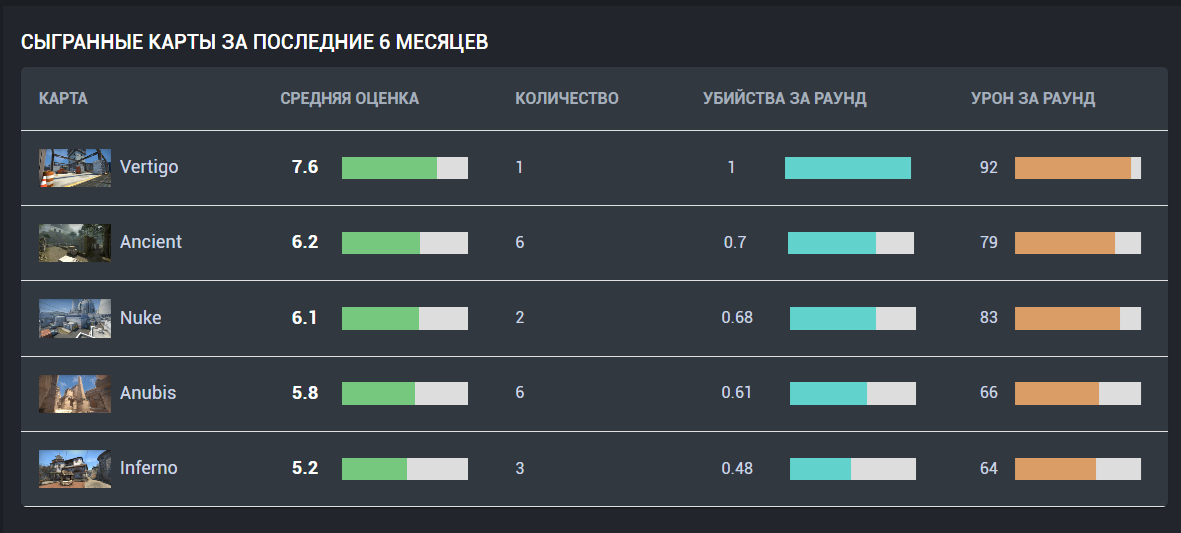
\includegraphics[width=0.95\linewidth]{images/MapStatsTable}
	\caption{Пример отображения компонента MapStatsTable}
	\label{fig:MapStatsTable}
\end{figure}

Компонент включает в себя:
\begin{itemize}
	\item \textbf{Таблица со статистикой}: Таблица отображает информацию по картам, включая их название, изображение, средний рейтинг, количество игр, KPR (киллы за раунд) и DPR (урон за раунд).
	\item \textbf{Прогресс-бары}: Прогресс-бары используются для визуализации средних значений рейтинга, KPR и DPR, обеспечивая наглядное представление данных.
\end{itemize}

Компонент реализован с использованием библиотеки Material UI и включает стиль, обеспечивающий удобство использования и хорошую визуализацию данных.

\paragraph{PlayerStats}

Компонент PlayerStats отображает статистику игроков в матче. Данный компонент представляет данные в виде таблицы, включающей следующие столбцы:

\begin{itemize}
	\item \textbf{Игрок}: Имя игрока и его аватар.
	\item \textbf{У}: Количество убийств.
	\item \textbf{С}: Количество смертей.
	\item \textbf{П}: Количество помощи (ассистов).
	\item \textbf{+/-}: Разница между убийствами и смертями.
	\item \textbf{СУ}: Среднее количество убийств за раунд.
	\item \textbf{ПД}: Позиция защиты.
	\item \textbf{МК}: Количество матчей, в которых игрок стал MVP.
	\item \textbf{1VSX}: Количество выигранных ситуаций 1 на X.
	\item \textbf{Рейтинг}: Оценка эффективности игрока.
	\item \textbf{Форма}: Изменение рейтинга формы игрока.
\end{itemize}

На рисунке \ref{fig:PlayerStats} представлен пример отображения компонента PlayerStats:

\begin{figure}
	\centering
	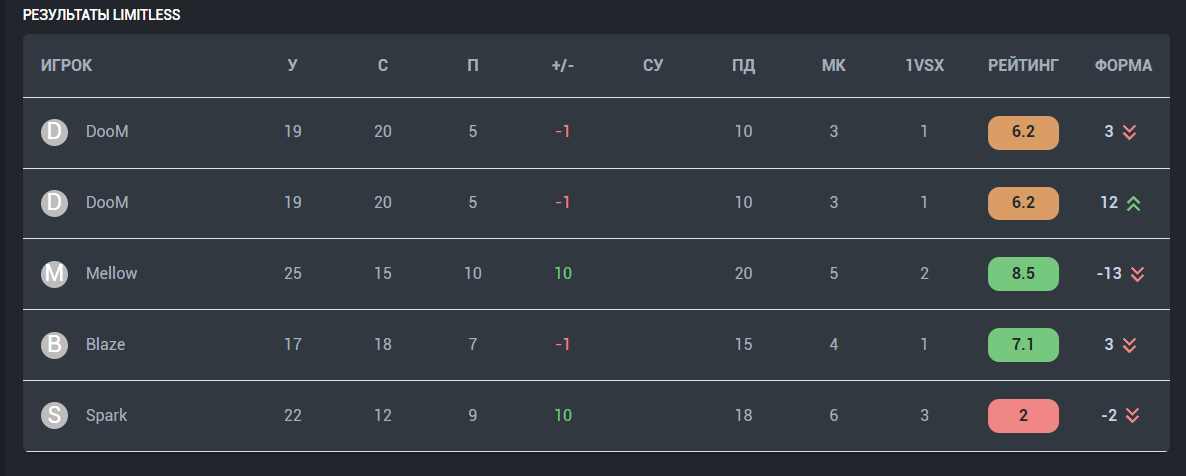
\includegraphics[width=0.95\linewidth]{images/PlayerStats}
	\caption{Пример отображения компонента PlayerStats}
	\label{fig:PlayerStats}
\end{figure}

Компонент включает в себя:
\begin{itemize}
	\item \textbf{Таблица со статистикой}: Таблица отображает информацию по игрокам, включая их имя, аватар, количество убийств, смертей, ассистов, рейтинг и форму.
	\item \textbf{Индикаторы изменений}: Используются индикаторы для отображения изменений в форме игрока.
\end{itemize}

Компонент реализован с использованием библиотеки Material UI.

\paragraph{MapPulStatsTable}

Компонент MapPulStatsTable отображает подробную статистику по картам, включая процент побед, количество сыгранных карт и другие метрики. Данный компонент представляет данные в виде таблицы, включающей следующие столбцы:

\begin{itemize}
	\item \textbf{Карта}: Название карты и изображение карты.
	\item \textbf{Процент побед}: Процент побед на данной карте, визуально представлен в виде прогресс-бара.
	\item \textbf{Количество}: Количество сыгранных карт.
	\item \textbf{Последние 5 карт}: Результаты последних пяти игр на данной карте.
	\item \textbf{Убийства за раунд}: Среднее количество убийств за раунд, визуально представленное прогресс-баром.
	\item \textbf{Урон за раунд}: Средний урон за раунд, визуально представлен в виде прогресс-бара.
\end{itemize}

На рисунке \ref{fig:MapPulStatsTable} представлен пример отображения компонента MapPulStatsTable:
\begin{figure}
	\centering
	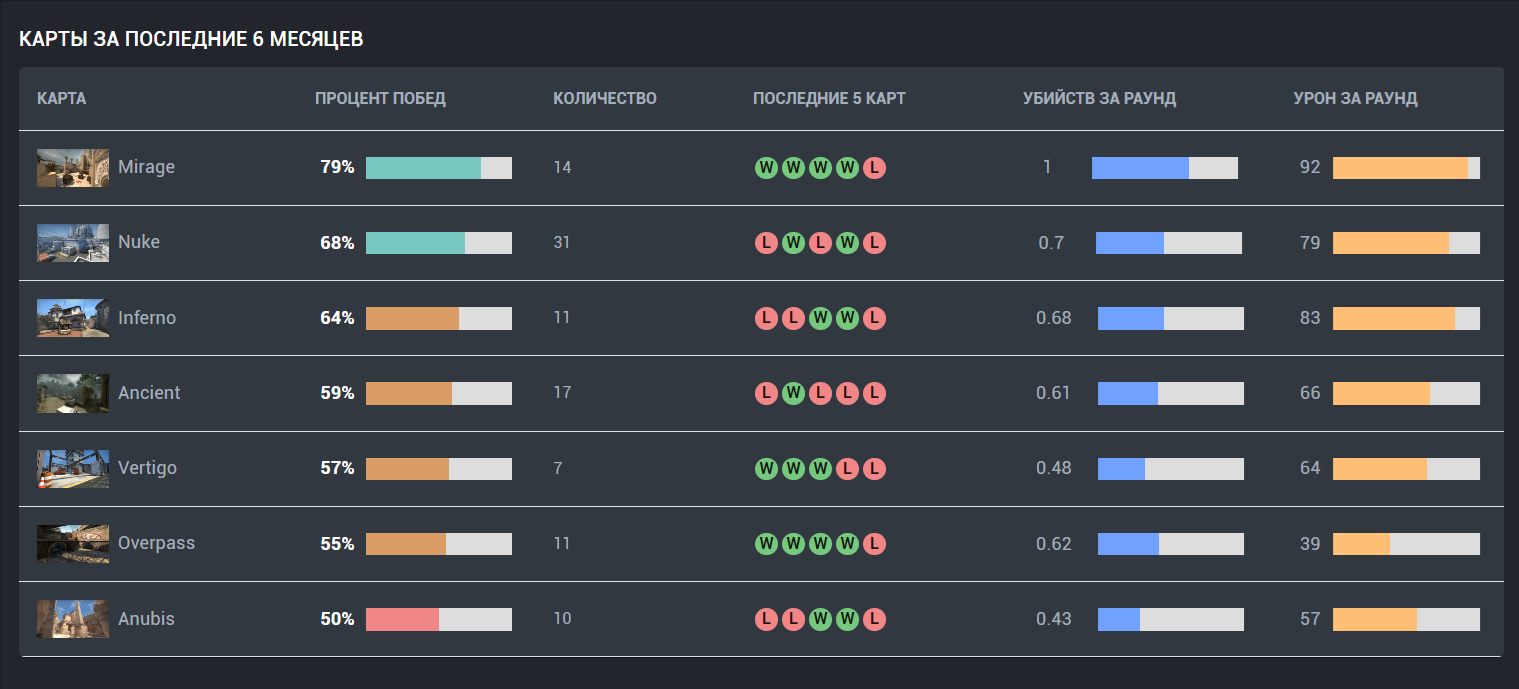
\includegraphics[width=0.95\linewidth]{images/MapPulStatsTable}
	\caption{Пример отображения компонента MapPulStatsTable}
	\label{fig:MapPulStatsTable}
\end{figure}

Компонент включает в себя:
\begin{itemize}
	\item \textbf{Таблица со статистикой}: Таблица отображает информацию по картам, включая их название, изображение, процент побед, количество игр, последние пять результатов игр, KPR (киллы за раунд) и DPR (урон за раунд).
	\item \textbf{Прогресс-бары}: Прогресс-бары используются для визуализации значений процента побед, KPR и DPR, обеспечивая наглядное представление данных.
\end{itemize}

Компонент реализован с использованием библиотеки Material UI и включает стиль, обеспечивающий удобство использования и хорошую визуализацию данных.